\begin{figure}[htbp]
\centering
\captionsetup{
  justification=raggedright,
  labelsep=none,
  singlelinecheck=false,
  labelformat=boldlabel,
}
\caption[Figure 1: \footnotesize ]{\footnotesize \textbf{: Net feature importance by theme across ML models (last period).} Net (signed sum of) normalized feature importance within each signal theme in the final out-of-sample period, for every ML model (OLS, GLMNET, RF, XGB, NN1--NN3). Feature importance is a global OLS surrogate of the model output on the same signals; because signals within a theme are highly correlated their coefficients offset, so importances are summed within each theme to recover the net contribution. Bars are coloured by sign; themes are ordered by overall net importance.}
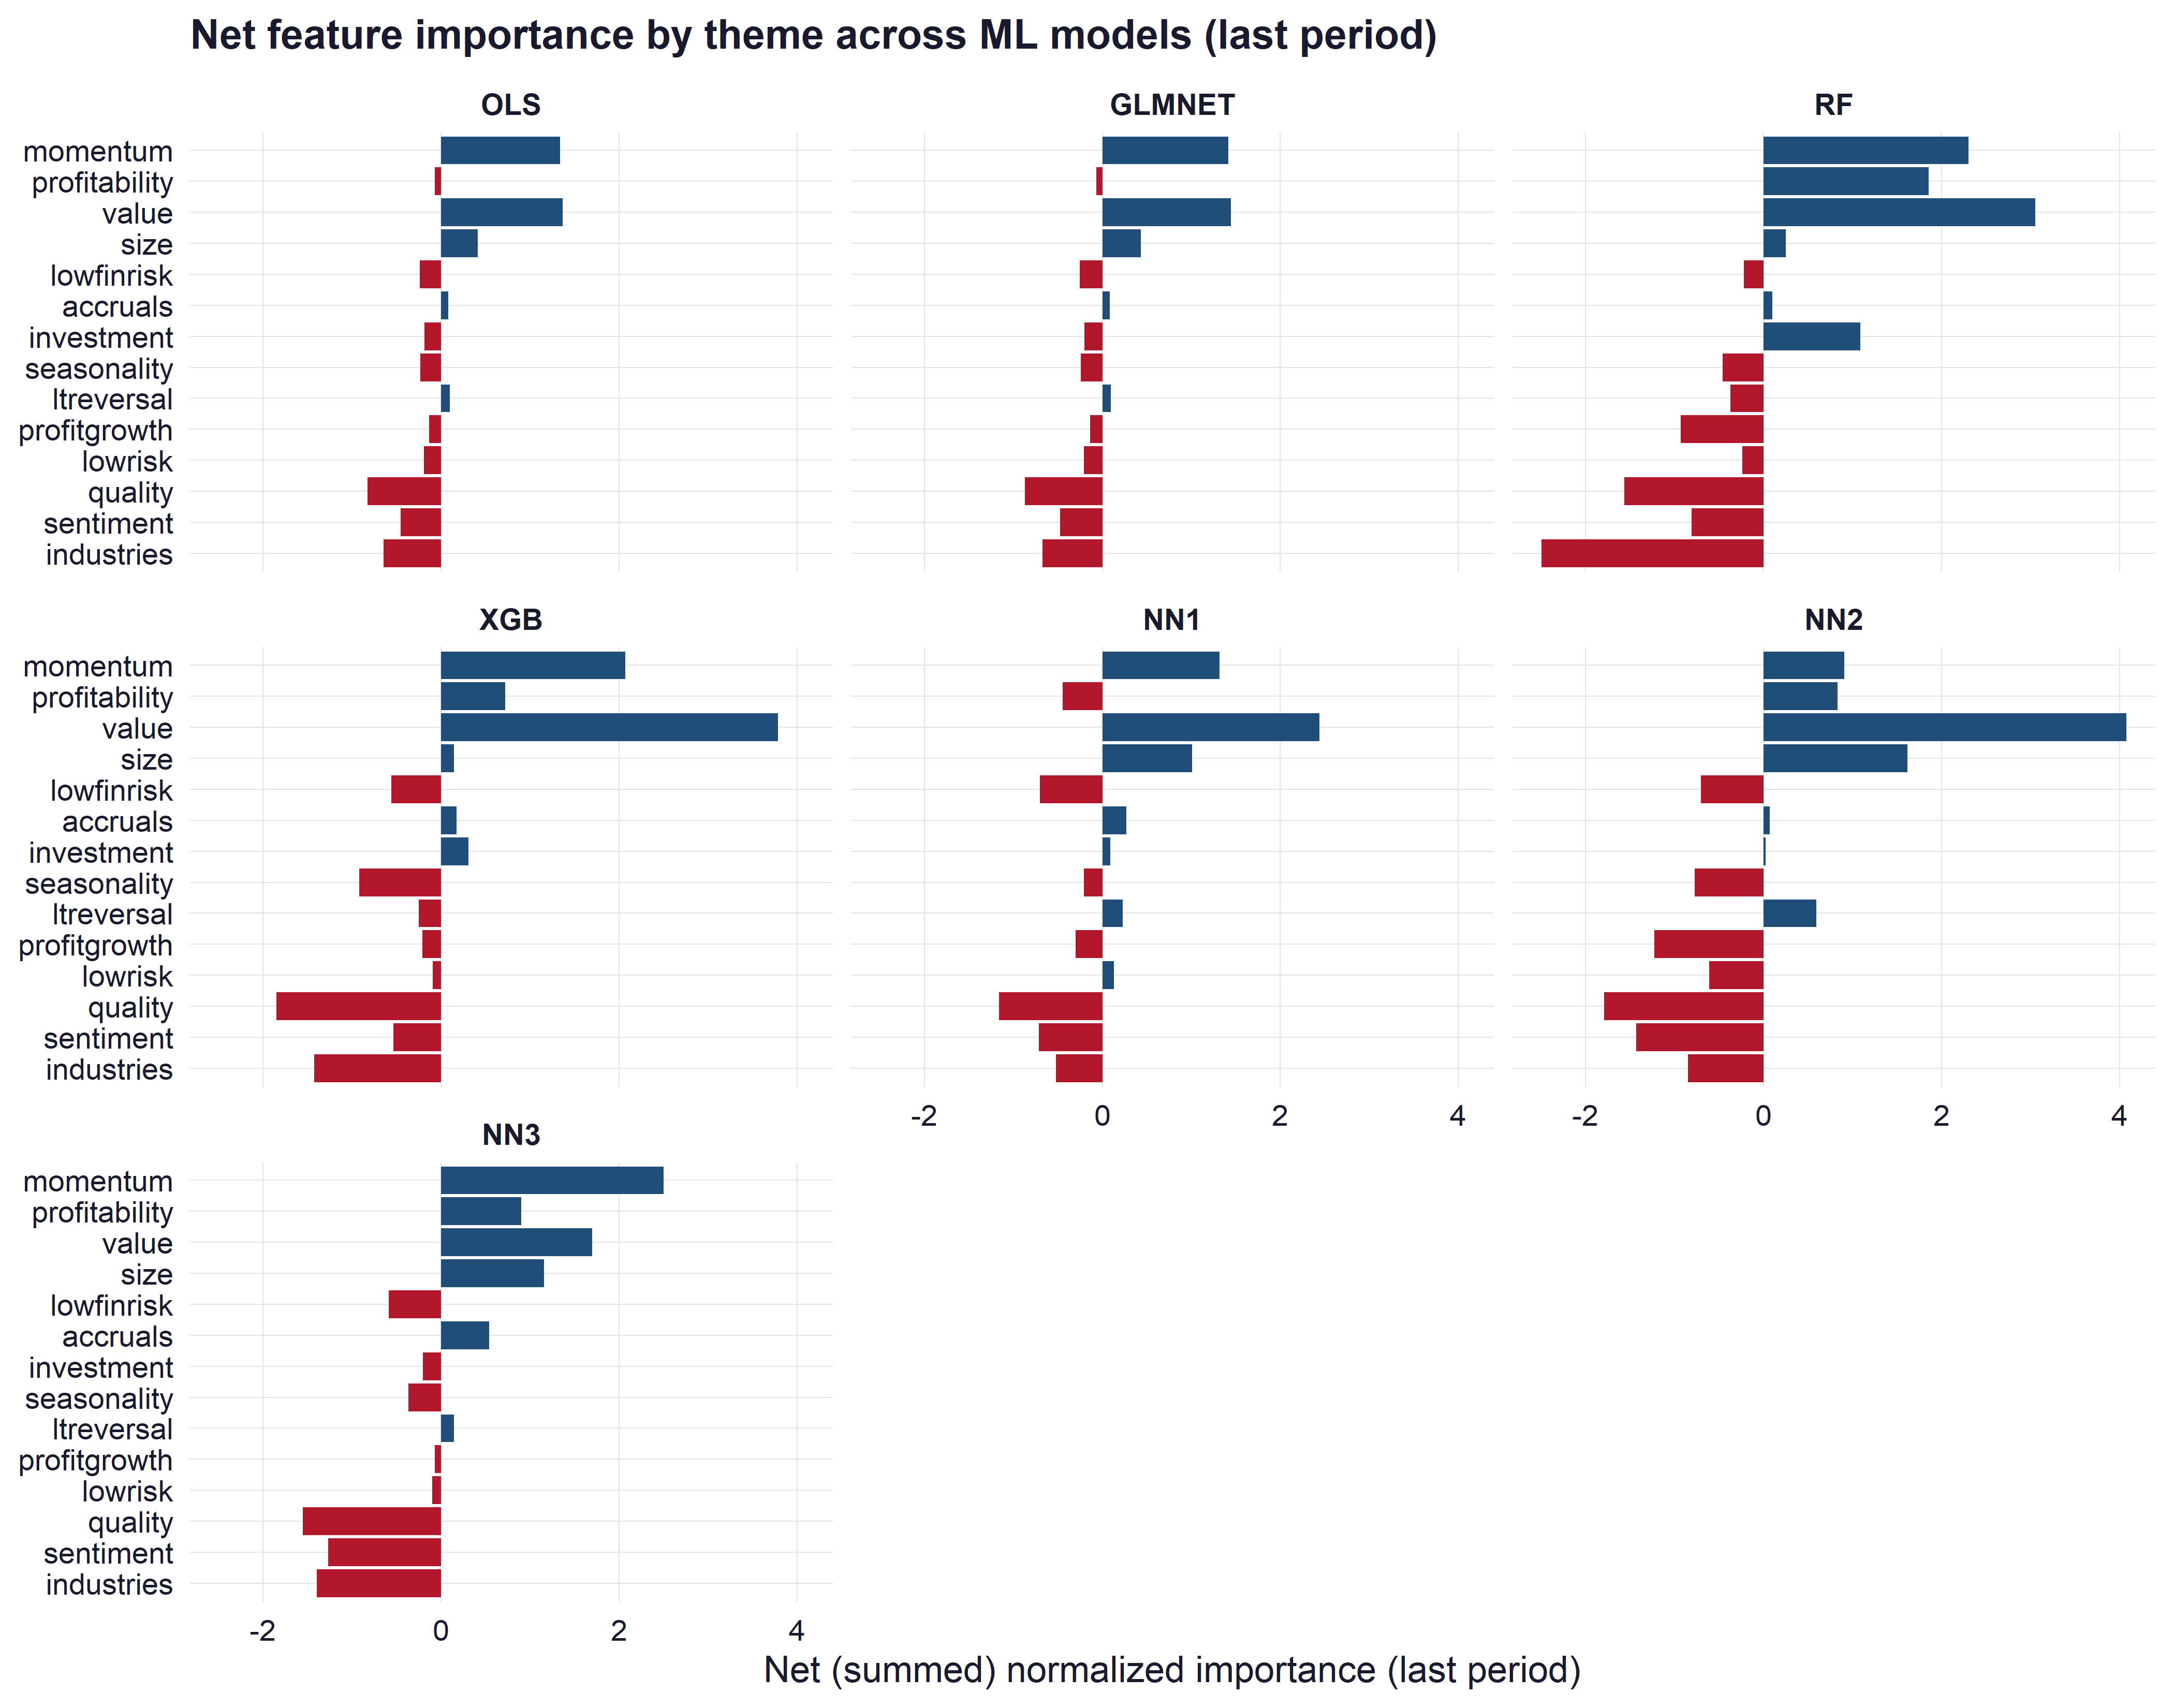
\includegraphics[width=\linewidth]{figures/feature_importance_bar.png}
\label{fig:fi_bar}
\end{figure}

\begin{figure}[htbp]
\centering
\captionsetup{
  justification=raggedright,
  labelsep=none,
  singlelinecheck=false,
  labelformat=boldlabel,
}
\caption[Figure 2: \footnotesize ]{\footnotesize \textbf{: Net feature importance by theme over time across ML models.} Net (signed sum of) normalized feature importance per signal theme at each rebalance date, for every ML model (OLS, GLMNET, RF, XGB, NN1--NN3). Each panel shows one model; colour encodes net importance on a diverging scale centred at zero. Themes are ordered by overall net importance.}
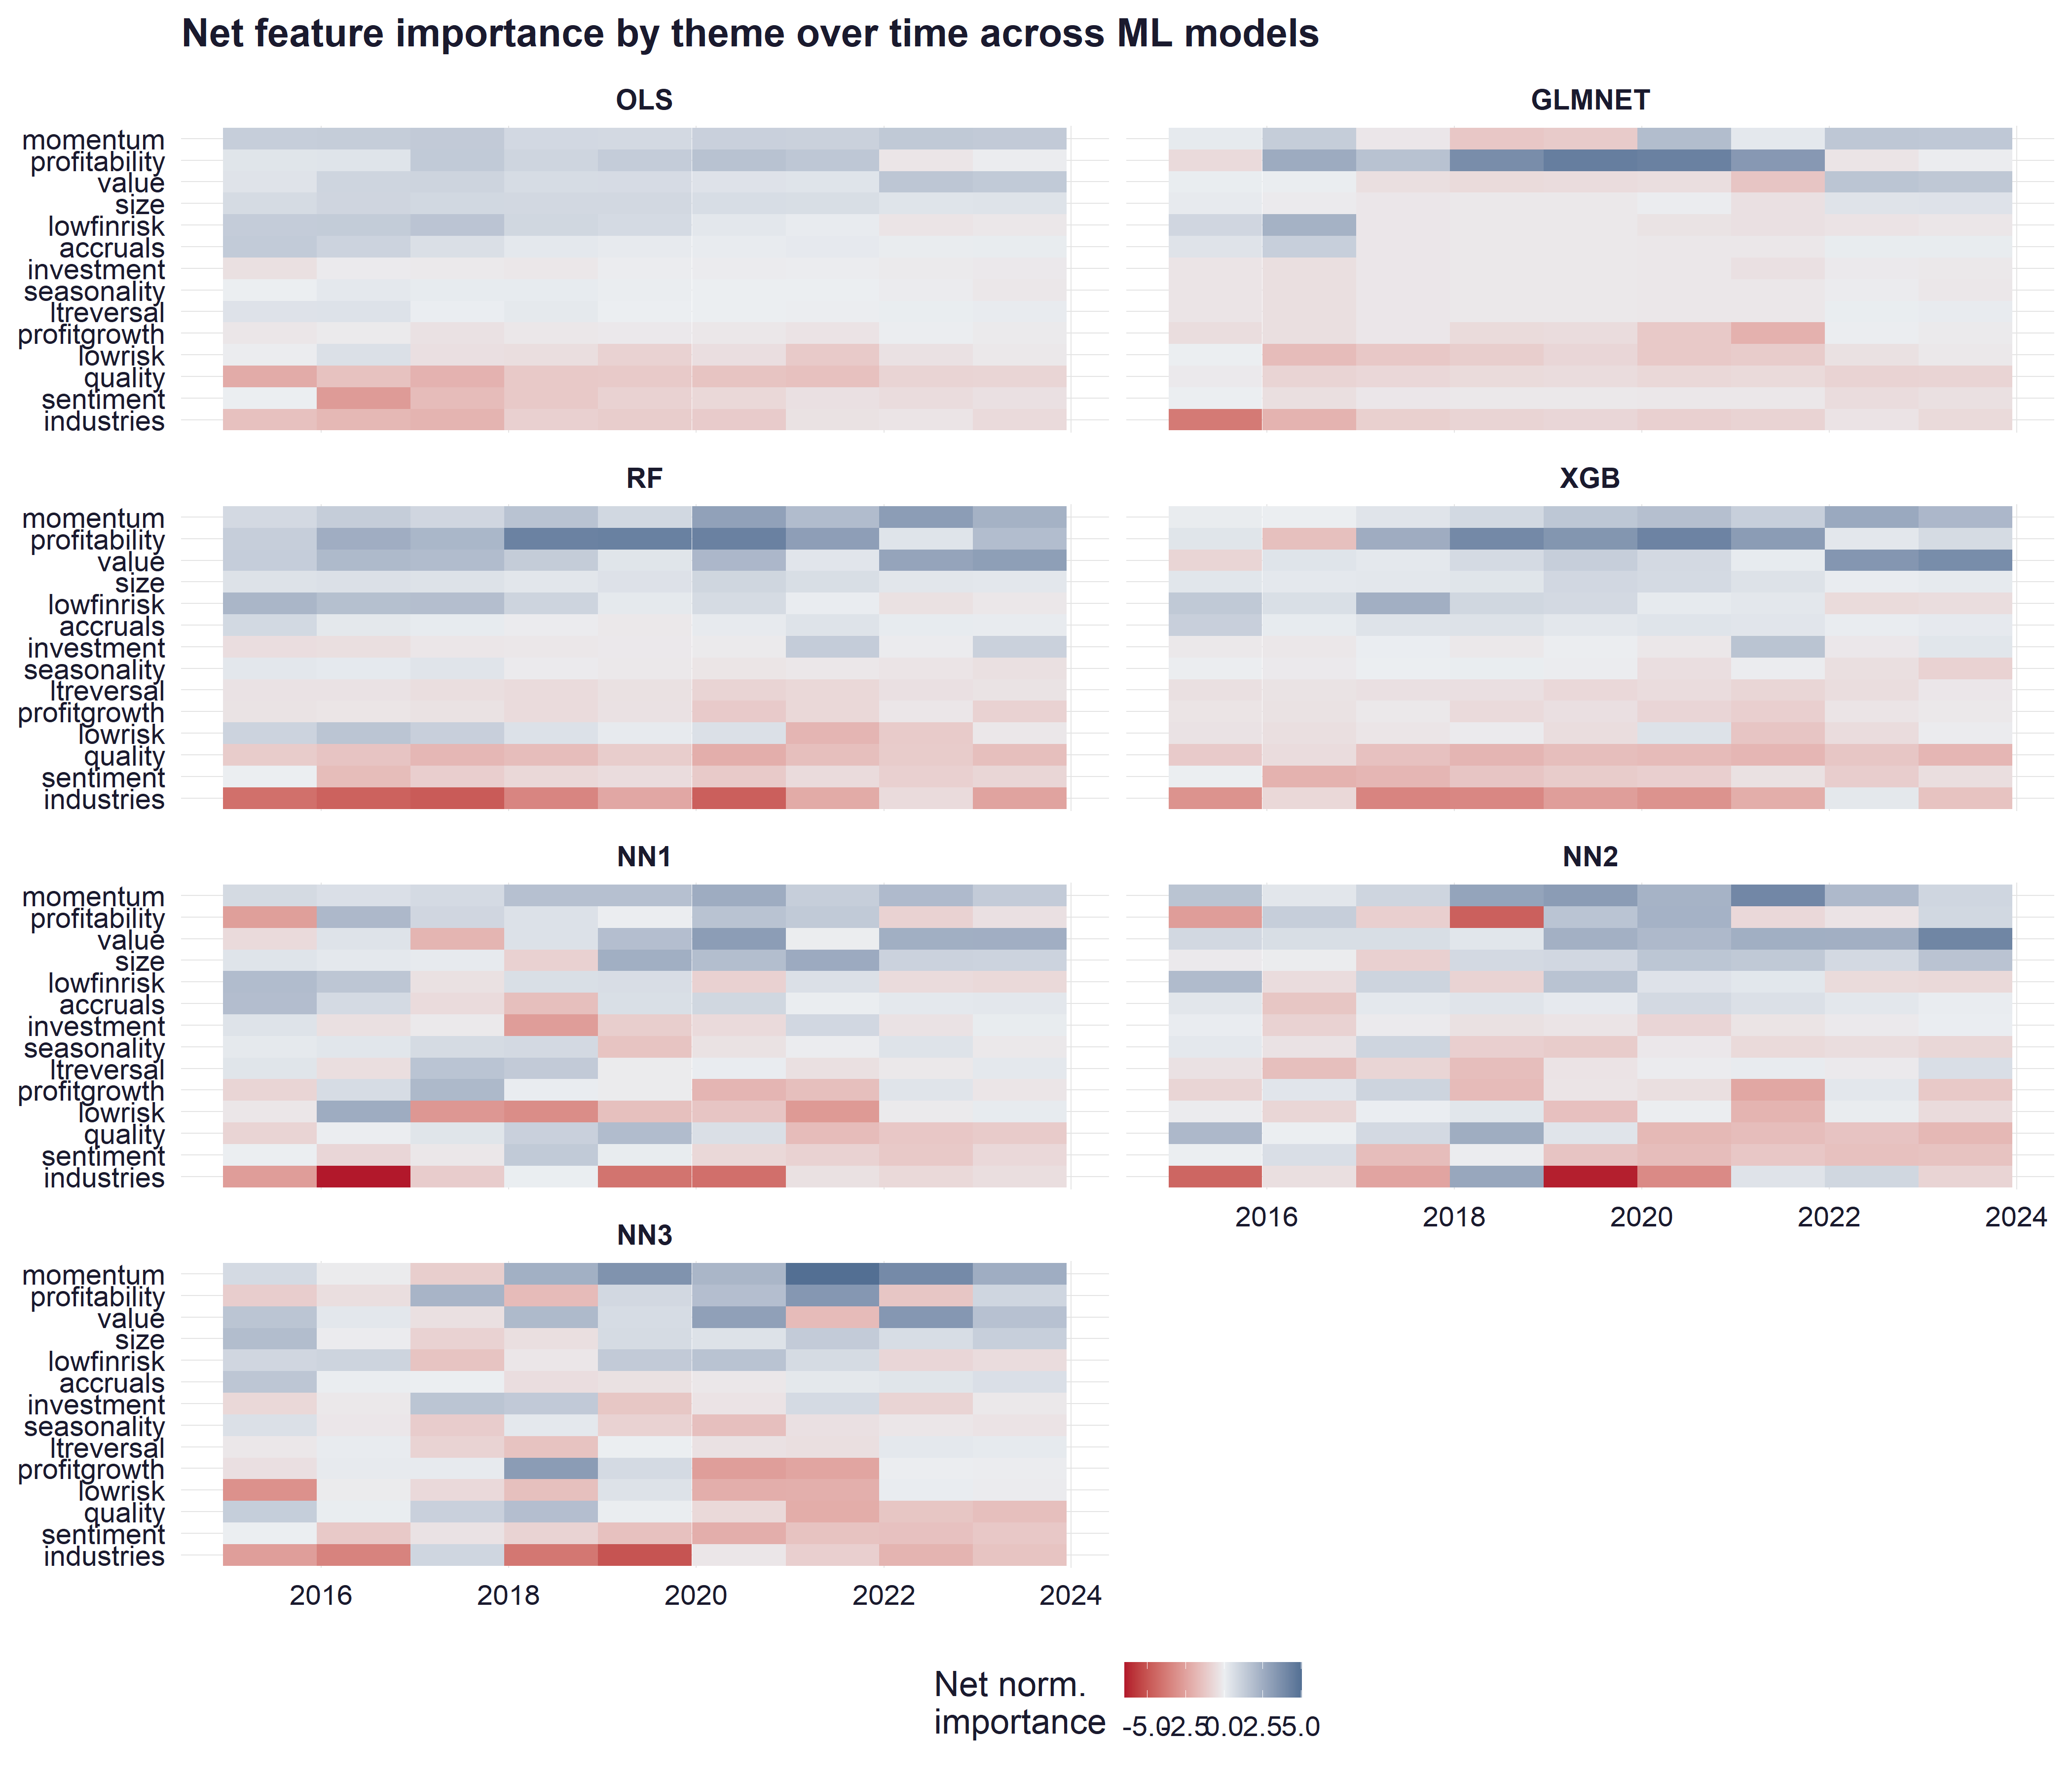
\includegraphics[width=\linewidth]{figures/feature_importance_heatmap.png}
\label{fig:fi_heatmap}
\end{figure}
